\begin{appendices}

\begin{figure}[!h]
  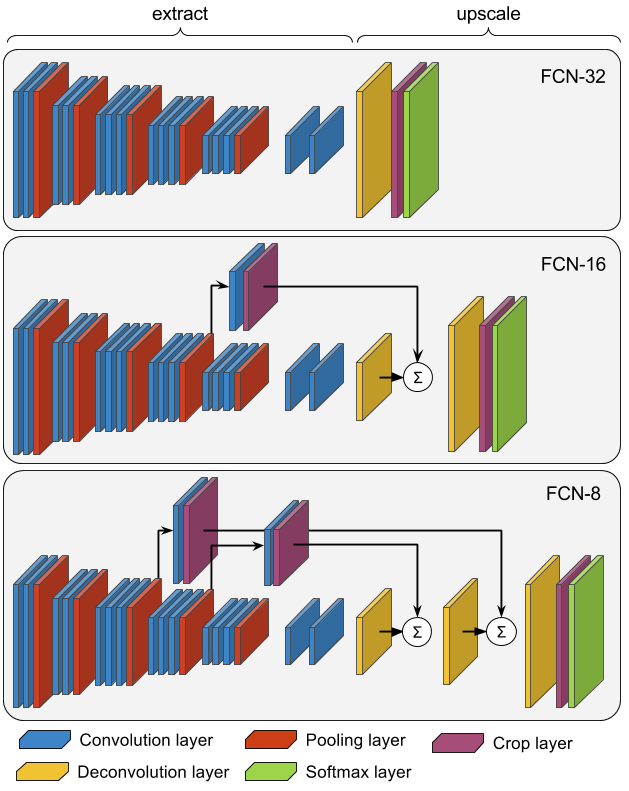
\includegraphics[width=1\linewidth,center]{images/appendices/fcns_architecture.png}
  \caption{Comparison of the three architectures of FCN}\textbf{
  \label{fig:appendices:fcns_architecture}}
\end{figure}

\todo{create with subfigures}
\begin{figure}[!h]
  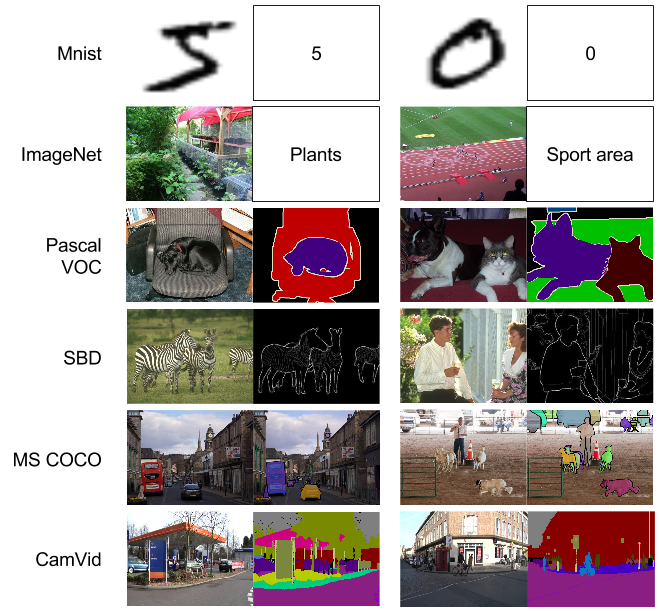
\includegraphics[width=1\linewidth,center]{images/appendices/datasets_comparison.png}
  \caption{Comparison of the most famous datasets}\textbf{
  \label{fig:appendices:datasets_comparison}}
\end{figure}

\begin{landscape}
\begin{table}[htbp]
  \centering
  \begin{tabular}{rcccccc}
    \rowcolor{gray!50}
    \toprule
    yop & yop & \textbf{Caffe~\footnote{caffe.berkeleyvision.org} Berkeley} & \textbf{CNTK~\footnote{cntk.ai} Microsoft} & \textbf{Tensorflow~\footnote{tensorflow.org} Google} & \textbf{Theano~\footnote{deeplearning.net/software/theano} Montreal Univ} & \textbf{Torch~\footnote{torch.ch} N.Y.U} \\
    \midrule
    Available pre-trained models (CNN) & LeNet  & V & X & X & V & V \\
    yop & AlexNet  & V & X & X & V & V \\
    yop & VGGs  & V & V & V & V & V \\
    yop & GoogleNet  & V & X & X & V & V \\
    yop & ResNet  & V & X & X & X & X \\
    yop  & SegNet  & V (C) & X & X & X & X \\
    yop  & FCNs  & V & X & X & X & X \\
    Speed (one GPU) & yop  & Fast & Fast & Slow & Fast & Very fast \\
    Number max of GPU & yop  & 4 & 8 & 4 & 2 & 2 \\
    CudNN compatibility & yop  & V & V & V & V & V \\
    Modelling capability & CNN & V & V & V & V & V \\
    yop & RNN & X & V & V & V & X \\
    yop & New models & X & V & V & V & V \\
    Readable source code & yop & V & X & X & X & V \\
    Interface & yop & Command line (pycaffe) & Command line & Python, C++ & Python & Lua \\
    Architecture & yop & Rigid & Quite modulable & Clean and modulable & Modulable but not intuitive & Clean and modulable \\
    \bottomrule
  \end{tabular}%
  
  \caption{Frameworks comparison}
  \label{appendices:frameworks_comparison}
\end{table}%
\end{landscape}

\todo{to complete}
\rowcolors{2}{gray!25}{white}
\begin{table}[htbp]
  \centering
  
  \begin{tabular}{rcccccc}
    \rowcolor{gray!50}
    \toprule
    \textbf{Architecture} & \textbf{Mean IU} & \textbf{fwIU} \\
    \midrule
    SegNet &				xx & 		xx \\
    FCN-32 &				xx & 		xx \\
    FCN-32-16 &			xx & 		xx \\
    FCN-32-16-8 &		xx & 		xx \\
    FCN-32-ResNet-50 &	xx & 		xx \\
    FCN-32-ResNet-101 &	xx & 		xx \\
    FCN-32-ResNet-152 &	xx & 		xx \\
    FCN-16-ResNet-50 &	xx & 		xx \\
    FCN-16-ResNet-101 &	xx & 		xx \\
    FCN-16-ResNet-152 &	xx & 		xx \\
    \bottomrule
  \end{tabular}%
  
  \caption{Comparison of the accuracy of different architectures on the Okutama dataset}
  \label{appendices:setup2:_oku}
\end{table}%


\end{appendices}